\chapter{Lec 09 - Linear Regression III}

\section{Comparison of Linear Regression with K-Nearest Neighbors}
Linear regression is an example of a parametric approach because it assumes a linear functional form for $f(X)$.  Parametric methods have several advantages. They are often easy to fit, because one need estimate only a small number of coefficients.  But parametric methods do have a disadvantage: by construction, they make strong assumptions about the form of $f(X)$. If the specified functional form is far from the truth, and prediction accuracy is our goal, then the parametric method will perform poorly.\\\\
In contrast, non-parametric methods do not explicitly assume a parametric form for $f(X)$, and thereby provide an alternative and more flexible approach for performing regression. Here we consider one of the simplest and best-known
non-parametric methods, \textit{K-nearest neighbors} regression (KNN regression).\\\\
Given a value for $K$ and a prediction point $x_0$, KNN regression first identifies the $K$ training observations that are closest to $x_0$, represented by $\mathcal{N}_0$. It then estimates $f(x_0)$ using the average of all the training responses in $\mathcal{N}_0$. In other words,
\[\hat{f}(x_0) = \frac{1}{K}\sum_{x_i \in \mathcal{N}_0} y_i\]
In general, the optimal value for $K$ will depend on the bias-variance tradeoff. A small value for $K$ provides the most flexible fit, which will
have low bias but high variance. This variance is due to the fact that the
prediction in a given region is entirely dependent on just one observation.
In contrast, larger values of $K$ provide a smoother and less variable fit; the
prediction in a region is an average of several points, and so changing one observation has a smaller effect. However, the smoothing may cause bias by masking some of the structure in $f(X)$.
\begin{center}
    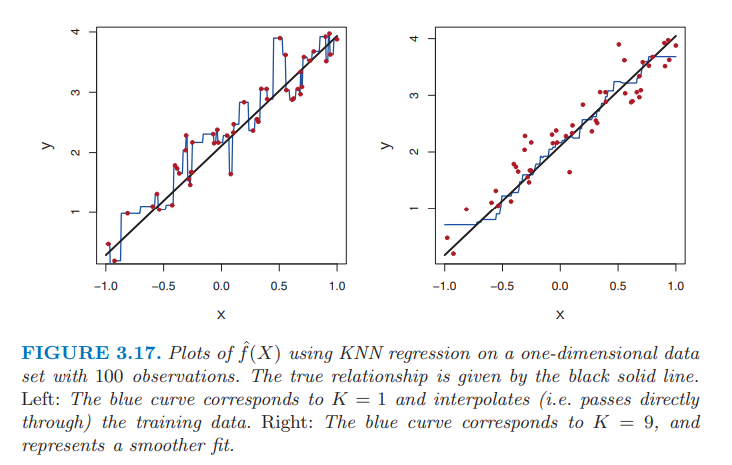
\includegraphics[scale=0.8]{images/linear-reg vs knn.png}
    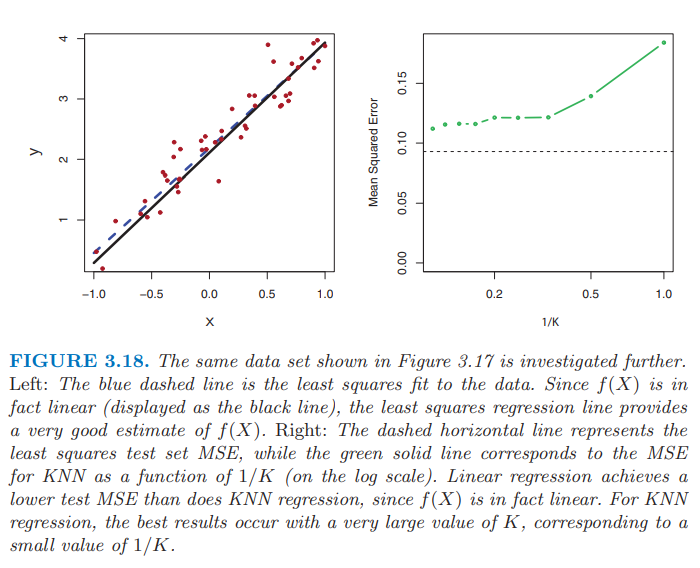
\includegraphics[scale=0.8]{images/knn.png}
\end{center}
The figures above provide an example with data generated from a one-dimensional linear regression model. The black solid lines represent $f(X)$, while the blue curves correspond to the KNN fits using $K = 1$ and $K = 9$. In this case, the $K = 1$ predictions are far too variable, while
the smoother $K = 9$ fit is much closer to $f(X)$. However, since the true
relationship is linear, it is hard for a non-parametric approach to compete with linear regression.
\begin{center}
    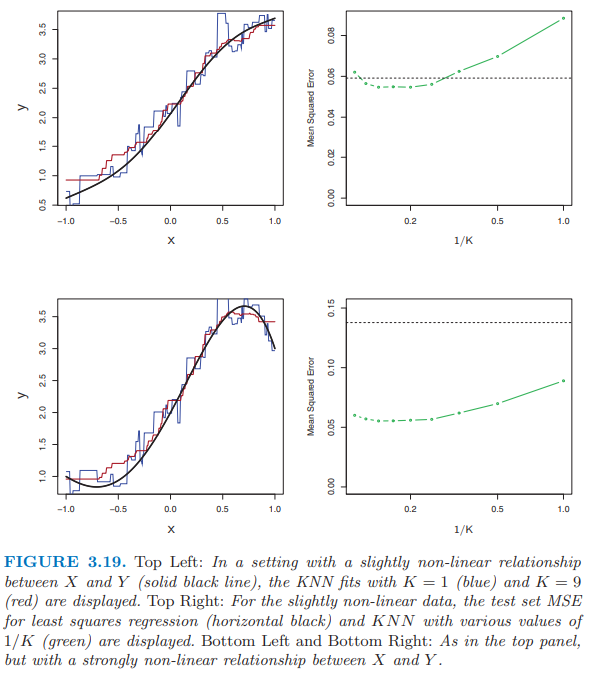
\includegraphics[scale=0.8]{images/linear-reg vs knn 2.png}
\end{center}
The figure above examines the relative performances of least squares regression and KNN under increasing levels of non-linearity in the relationship
between $X$ and $Y$ . In the top row, the true relationship is nearly linear.
In this case we see that the test MSE for linear regression is still superior
to that of KNN for low values of $K$. However, for $K \geq 4$, KNN outperforms linear regression. The second row illustrates a more substantial deviation from linearity. In this situation, KNN substantially outperforms linear regression for all values of $K$.\\\\
When $p = 1$ or $p = 2$, KNN outperforms linear regression. But for $p = 3$ the results are mixed, and for $p \geq 4$ linear regression is superior to KNN. This is caused by the curse of dimensionality that we already discussed.
\begin{center}
    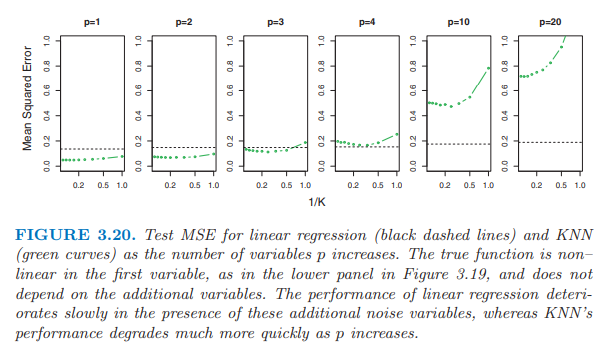
\includegraphics[scale=0.8]{images/curse of dim.png}
\end{center}
Even in problems in which the dimension is small, we might prefer linear regression to KNN from an interpretability standpoint.
